\input qpd-bootstrap

\begin{problem}{20260802}
  \meta{name}{Electromagnetic in Disk}
  \meta{setter}{Postulate V}
  \meta{score}{5}
  \meta{topic}{electromagnetism}
  \meta{difficulty}{3}
  \meta{tags}{electromagnetism, magnetic field, circular motion, Lorentz force}

Consider the annular region $R_1 \le r \le R_2$ in cylindrical coordinates $(r, \phi, z)$.  A uniform magnetic field
\[
  \mathbf{B} = B\,\hat{\mathbf{k}},
\]
directed upward, fills this region.



\begin{center}
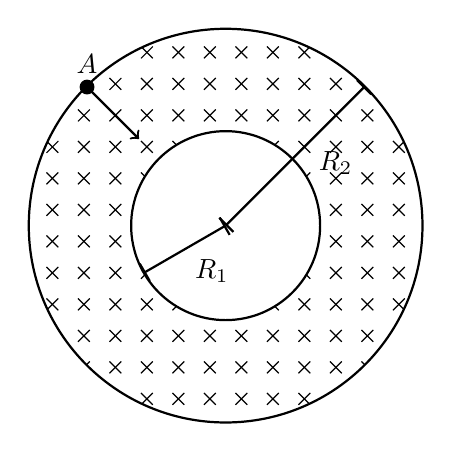
\begin{tikzpicture}

    \def\rInner{1.2}
    \def\rOuter{2.5}
    \def\s{0.075} % Cross half-size radius

    % 1. Draw boundary circles
    \draw[thick] (0,0) circle (\rInner);
    \draw[thick] (0,0) circle (\rOuter);

    % 2. Render field crosses inside the annulus only, via a real clip.
    % Uses the PGF-level even-odd rule (outer + inner circle) to cut the hole;
    % TikZ's \clip does not support `even odd rule`/`reverse path` on this
    % PGF version, but the low-level \pgfseteorule primitive does.
    \begin{scope}
        \pgfseteorule
        \pgfpathcircle{\pgfpointorigin}{\rOuter cm}
        \pgfpathcircle{\pgfpointorigin}{\rInner cm}
        \pgfusepath{clip}
        \foreach \x in {-2.6, -2.2, ..., 2.6} {
            \foreach \y in {-2.6, -2.2, ..., 2.6} {
                \draw[thin] (\x-\s, \y-\s) -- (\x+\s, \y+\s);
                \draw[thin] (\x-\s, \y+\s) -- (\x+\s, \y-\s);
                }
            }
    \end{scope}

    % Entry point A on the outer circle, with the velocity vector directed
    % radially inward toward the axis.
    \draw[thick, fill=black] (-1.76, 1.76) circle (0.08);
    \node at (-1.76, 2.05) {$A$};
    \draw[->, thick] (-1.76, 1.76) -- (-1.10, 1.10);

    % Dimension lines for the two radii, drawn at different angles (not
    % colinear): R_1 to the inner circle, R_2 to the outer circle.
    \draw[|-|, thick] (0,0) -- (210:1.2) node[midway, below right] {$R_1$};
    \draw[|-|, thick] (0,0) -- (45:2.5);
    \node at (45:1.5) [below right] {$R_2$};

\end{tikzpicture}
\end{center}

A particle of mass $m$ and charge $q$ enters the region at a point $A$ on the outer circle $r = R_2$, with speed $v$ directed radially inward toward the axis. The particle traces through a trajectory tangent to the inner circle $r = R_1$, subsequently leaves the region, and never enters it again.

\begin{questions}
  \item Find $B$ in terms of $m$, $q$, $v$, $R_1$, and $R_2$.
\end{questions}

\end{problem}

\begin{solution}{20260802}

\begin{center}
\begin{tikzpicture}[line cap=round, line join=round]
  \def\rInner{1.2}
  \def\rOuter{2.5}
  \def\s{0.075} % Cross half-size radius

  % 1. Draw boundary circles
  \draw[thick] (0,0) circle (\rInner);
  \draw[thick] (0,0) circle (\rOuter);

  % 2. Render field crosses inside the annulus only, via a real clip.
  \begin{scope}
    \pgfseteorule
    \pgfpathcircle{\pgfpointorigin}{\rOuter cm}
    \pgfpathcircle{\pgfpointorigin}{\rInner cm}
    \pgfusepath{clip}
    \foreach \x in {-2.6, -2.2, ..., 2.6} {
        \foreach \y in {-2.6, -2.2, ..., 2.6} {
            \draw[thin] (\x-\s, \y-\s) -- (\x+\s, \y+\s);
            \draw[thin] (\x-\s, \y+\s) -- (\x+\s, \y-\s);
            }
        }
  \end{scope}

  % 3. The auxiliary triangle A-O'-O: a right triangle at A with legs
  %    OA = R_2, AO' = R' and hypotenuse OO' = R' + R_1.  Its sides encode
  %    (R' + R_1)^2 = R_2^2 + R'^2, i.e. R' = (R_2^2 - R_1^2)/(2 R_1).
  \draw[gray!50!black, thick] (0,0) -- (0,2.5) -- (-2.004,2.5) -- cycle;

  %    Axis dot O at the centre.
  \fill (0,0) circle[radius=1.8pt] node[below left] {$O$};

  % 4. Particle orbit: a full circle of radius R' = (R_2^2 - R_1^2)/(2 R_1),
  %    centred at (-R', R_2) so that it passes through A = (0, R_2) and is
  %    tangent to the inner circle.  The arc the particle actually traces is
  %    solid; the remainder of the circle is dashed.
  \draw[gray, very thick, -{Stealth}] (0, 2.5)
      arc[start angle=0, end angle=-102.56, radius=2.004];
  \draw[blue, very thick, dashed] (-2.4401, 0.5438)
      arc[start angle=-102.56, end angle=-360, radius=2.004];

  %    Orbit centre and tangency/exit points.
  \fill[black] (-2.004, 2.5) circle[radius=1.6pt] node[above left] {$O'$};
  \fill[black] (-0.7506, 0.9363) circle[radius=1.6pt] node[below] {$T$};
  \fill[black] (-2.4401, 0.5438) circle[radius=1.6pt] node[below left] {$B$};

  % 5. Entry point A on the outer circle, velocity directed radially inward.
  \draw[thick, fill=black] (0, 2.5) circle (0.08);
  \node at (-.4, 2.92) {$A$};
  \draw[->, thick] (0, 2.5) -- (0, 1.7);

\end{tikzpicture}

\end{center}

\subsection*{Q1. Magnetic Field}

The particle experiences the Lorentz force
\[
  \mathbf{F} = q\,\mathbf{v}\times\mathbf{B}.
\]
Taking the entry point on the $+y$-axis, the inward velocity is $\mathbf{v} = -v\,\hat{\mathbf{j}}$ while $\mathbf{B} = B\,\hat{\mathbf{k}}$, so
\[
  \mathbf{F} = q\,(-v\hat{\mathbf{j}})\times(B\hat{\mathbf{k}})
            = -qvB\,(\hat{\mathbf{j}}\times\hat{\mathbf{k}})
            = -qvB\,\hat{\mathbf{i}}.
\]
For $q>0$ the force points along $-\hat{\mathbf{i}}$, so the orbit bends to the left; for $q<0$ it bends to the right.  These are the two cases, and they give the same magnitude of $B$.

The force is purely centripetal, so the particle moves on a circle of gyroradius $\rho$ with
\[
  \frac{mv^2}{\rho} = \abs{q}vB
  \qquad\Longrightarrow\qquad
  \rho = \frac{mv}{\abs{q}B}.
\]

Let $O'$ be the centre of this circle and $T$ its point of tangency with the inner circle $r = R_1$.  The velocity at $A$ is radial, so $O'A \perp OA$ and the triangle $O\,A\,O'$ is right-angled at $A$, with
\[
  OA = R_2, \qquad AO' = \rho, \qquad OO' = \rho + R_1,
\]
the last because $OO'$ is the sum of the two touching radii $\rho$ and $R_1$.  Pythagoras then gives
\[
  (\rho + R_1)^2 = R_2^2 + \rho^2
  \;\Longrightarrow\;
  2\rho R_1 = R_2^2 - R_1^2
  \;\Longrightarrow\;
  \rho = \frac{R_2^2 - R_1^2}{2R_1}.
\]

Equating the two expressions for $\rho$ and solving for $B$,
\[
  \frac{mv}{\abs{q}B} = \frac{R_2^2 - R_1^2}{2R_1}
  \;\Longrightarrow\;
  \boxed{\,B = \frac{2mvR_1}{\abs{q}\,(R_2^2 - R_1^2)}\,}.
\]

\end{solution}

\input qpd-end
